\subsection{Randomness Analysis}
\label{sec:evaluation-randomness-analysis}
The randomness degree of the adopted pseudo-random number generator has been evaluated with the following standard tests:

\begin{itemize}
	\item \textbf{Spectral Test:} this test is considered one of the most intuitive and widely adopted tests to assess the quality of linear congruential generators \cite{knuth1981art}. 
	It relies on the fact that the output of such generators form lines or hyperplanes when plotted on 2 or more dimensions. The less the distance between these lines or planes, the better is the generator. 
	In fact, a smaller distance between lines or planes highlights a better uniform distribution.
	
	In Figure~\ref{fig:evaluation-randomness-spectral-16807},\ref{fig:evaluation-randomness-spectral-48271} and \ref{fig:evaluation-randomness-spectral-50812} we show the test results for generators $(16807,2^{31}-1)$, $(48271,2^{31}-1)$ and $(50812,2^{31}-1)$, respectively.

	The results show that the adopted generator $(50812,2^{31}-1)$ is much better than $(16807, 2^{31}-1)$, which has been widely adopted in the past, and it is really similar to $(48271,2^{31}-1)$, which is the current 32-bit de-facto standard, according to \cite{leemis2006discrete}.
	
	\item \textbf{Test of Extremes:} this test relies on the fact that if $U=U_{0},...,U_{d-1}$ is an independent identically distributed sequence of $Uniform(0,1)$ random variables, then $\max(U)^{d}$ is also a $Uniform(0,1)$. The test leverages this property to measures, for every stream, how much the generated random values differ from the theoretical uniform distribution.
	
	Given a number of streams $s$ and a level of confidence $c=1-\alpha$, the more the total number of fails is close to the expected value $s \cdot \alpha$, the better is the generator.
	
	In Figure~\ref{fig:evaluation-randomness-extremes-50812} we show the results for the adopted generator $(508012,2^{31}-1, 256)$ with sample size $n=10000$, $k=1000$ bins, sequence size $d=5$ and $95\%$ level of confidence.
	
	The adopted generator shows critical values $v_{min}=913$ and $v_{max}=1088$ and $14$ total fails ($7$ lower and $7$ upper fails), that is not far from the theoretical accepted number of fails, i.e. $256*0.05=13$.
	The proposed generator successfully passed the test with a $94.531\%$ level of confidence.
	
	\item \textbf{Kolmogorov-Smirnov Test:} the test measures, at a given level of confidence, the biggest vertical distance between the theoretical cumulative distribution function and the empirical cumulative distribution function.
	The more the recorded distance $d$ is less than the critical value $d^*$ for the considered level of confidence, the better the generator is.
	As the Kolmogorov-Smirnov analysis relies on pre-calculated randomness statistics, we have chosen to take into account the statistics obtained by the previous Test of Extremes.
	
	In Figure~\ref{fig:evaluation-randomness-kolmogorov-smirnov-50812} we show the test results for the proposed generator $(50812,2^{31}-1, 256)$ with a $95\%$ level of confidence.
	%
	The proposed generator successfully passed the test, as $d=0.041<0.081=d^*$.
	
\end{itemize}

We can conclude that the adopted generator $(50812,2^{31}-1, 256)$ provides a satisfying randomness degree.

\begin{figure}
	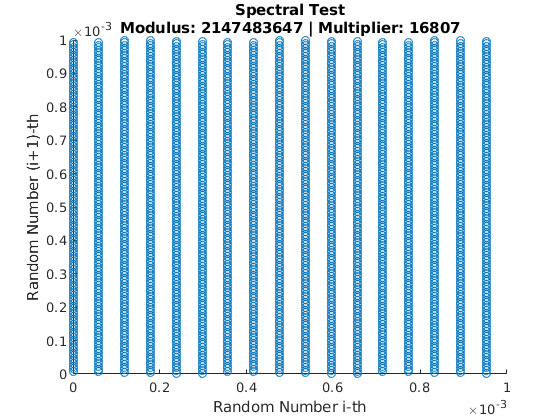
\includegraphics[width=\columnwidth]{fig/evaluation-randomness-spectral-16807}
	\caption{The Spectral Test for the generator $(16807,2^{31}-1, 1)$ in the interval $(0, 10^{-3})$.}
	\label{fig:evaluation-randomness-spectral-16807}
\end{figure}

\begin{figure}
	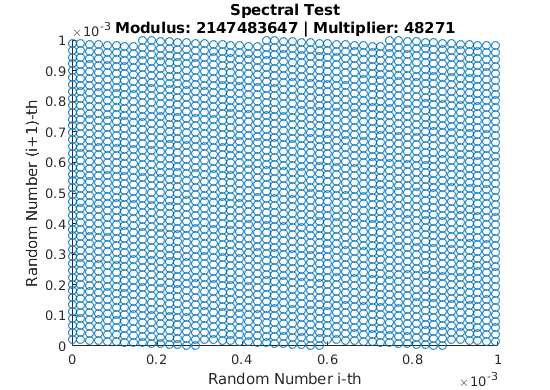
\includegraphics[width=\columnwidth]{fig/evaluation-randomness-spectral-48271}
	\caption{The Spectral Test for the generator $(48271,2^{31}-1, 1)$ in the interval $(0, 10^{-3})$.}
	\label{fig:evaluation-randomness-spectral-48271}
\end{figure}

\begin{figure}
	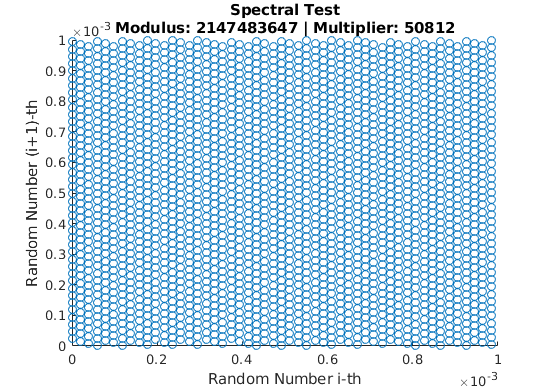
\includegraphics[width=\columnwidth]{fig/evaluation-randomness-spectral-50812}
	\caption{The Spectral Test for the generator $(50812,2^{31}-1, 1)$ in the interval $(0, 10^{-3})$.}
	\label{fig:evaluation-randomness-spectral-50812}
\end{figure}

\begin{figure}
	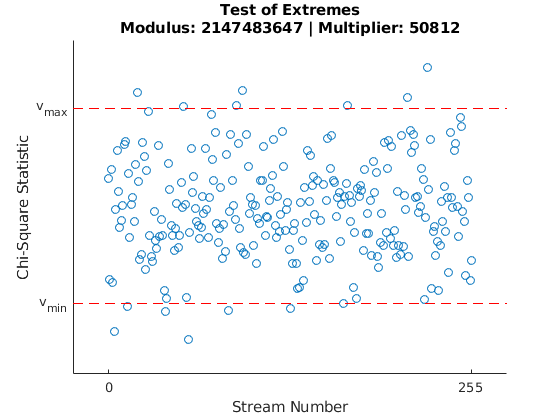
\includegraphics[width=\columnwidth]{fig/evaluation-randomness-extremes-50812}
	\caption{The Test of Extremes with $d=5$ to evaluate the randomness of the random number generator $(50812,2^{31}-1, 256)$.}
	\label{fig:evaluation-randomness-extremes-50812}
\end{figure}

\begin{figure}
	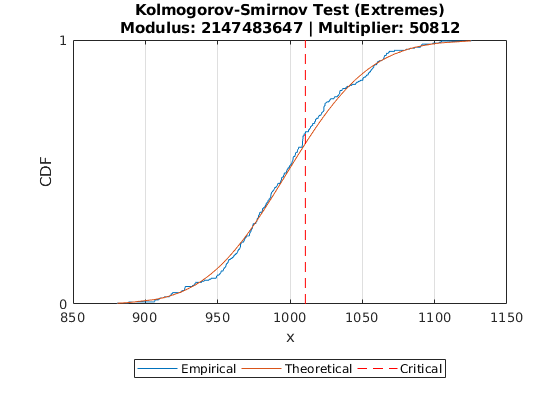
\includegraphics[width=\columnwidth]{fig/evaluation-randomness-kolmogorov-smirnov-50812}
	\caption{The Kolmogorov-Smirnov Analysis (leveraging the Test of Extremes with $d=5$) to evaluate the randomness of the random number generator $(50812,2^{31}-1, 256)$ with $95\%$ confidence.}
	\label{fig:evaluation-randomness-kolmogorov-smirnov-50812}
\end{figure}